\part{Laboratory Session 06}

\section*{Introduction}
In this laboratory unit the model of an inverse pendulum on a moving cart will be implemented snd simulated in simulink. In a first step the non linear model will be implemented and then discretized. After that the non linear model shall be linearized and discretized again. The differences between the two models are to be investigated. The two models shall be controlled with a PID controller. If the simulation works the model shall be deployed onto an actual moving robot to see if it holds up in real life.
 
\newpage
\section{Description of the Model}
The model consists of a moving part with a hinged pendulum atop. The goal for the controller is to accelerate the cart in the right direction depending on the angle of the pendulum in order to keep it upright at all times. 
\begin{figure}[H]
		\centering
		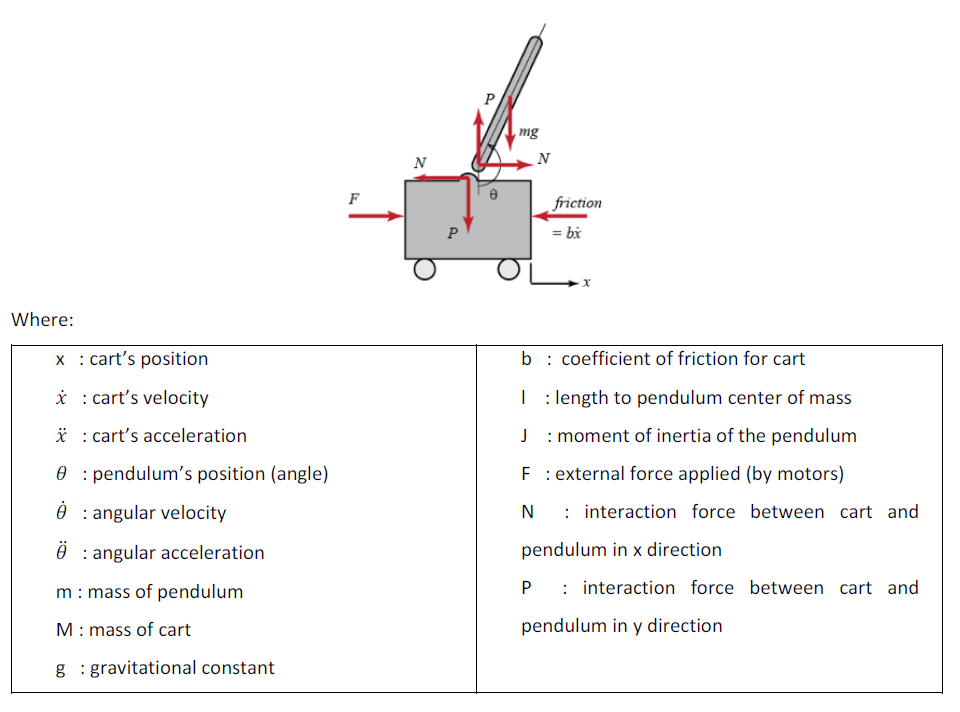
\includegraphics[width=0.7\textwidth]{figures/cart.png}
		\caption{graphical description of the model}
		\label{fig:scheme}
\end{figure}

The equations of the model are given by: 

	\begin{eqnarray}
		\ddot{x} &=& \frac{1}{M} \sum_{cart} F_x = \frac{1}{M} \left( F - N - b\dot{x}\right)  \\
		\ddot{\Theta} &=& \frac{1}{I} \sum_{pend} \tau = \frac{1}{I} \left( -Nlcos\Theta - Plsin\Theta \right)  \\
		N &=& m\left( \ddot{x} - l\dot{\Theta}^2 sin\Theta + l\ddot{\Theta}cos\Theta\right)  \\
		P &=& m\left( l\ddot{\Theta}^2cos\Theta + l\ddot{\Theta}sin \Theta\right) 
	\end{eqnarray}
\newpage	
\subsection{Implementation in simulink}
The non linear model can be implemented using the equations above, this was already done in a previous lectore in the third semester. The resulting model can be seen in Figure~\ref{fig:non_linear_continuous}.
\begin{figure}[H]
		\centering
		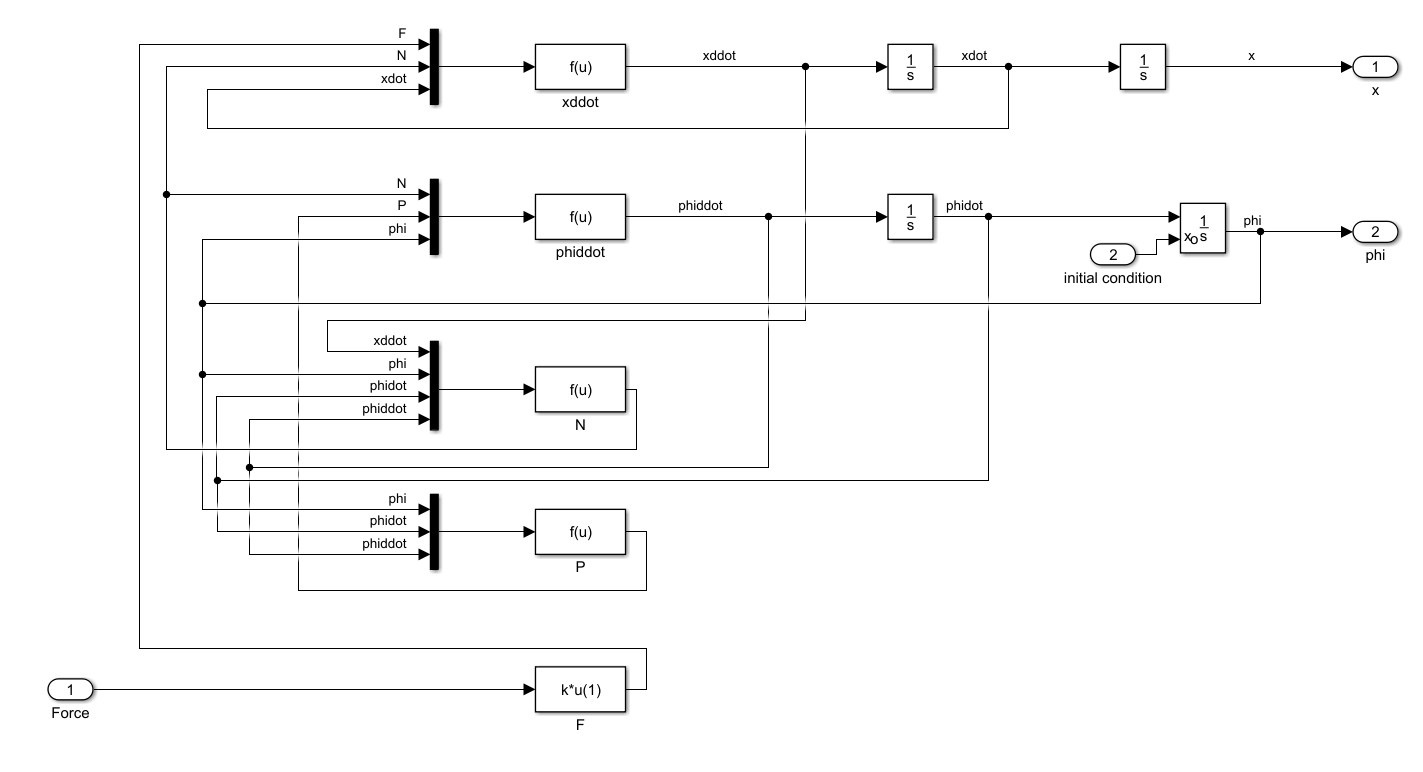
\includegraphics[width=0.7\textwidth]{figures/non_linear_continuous.png}
		\caption{Non linear continuous model in simulink}
		\label{fig:non_linear_continuous}
\end{figure}

\newpage
\section{Discretization from non-linear model}
Since the model will later be used on an actual hardware, it is important to sicretize the system. This is done by simply replacing the continuous time integrators with discrete time integrators. The settings of the integrators are shown in Figure~\ref{fig:integrator}.	
\begin{figure}[H]
		\centering
		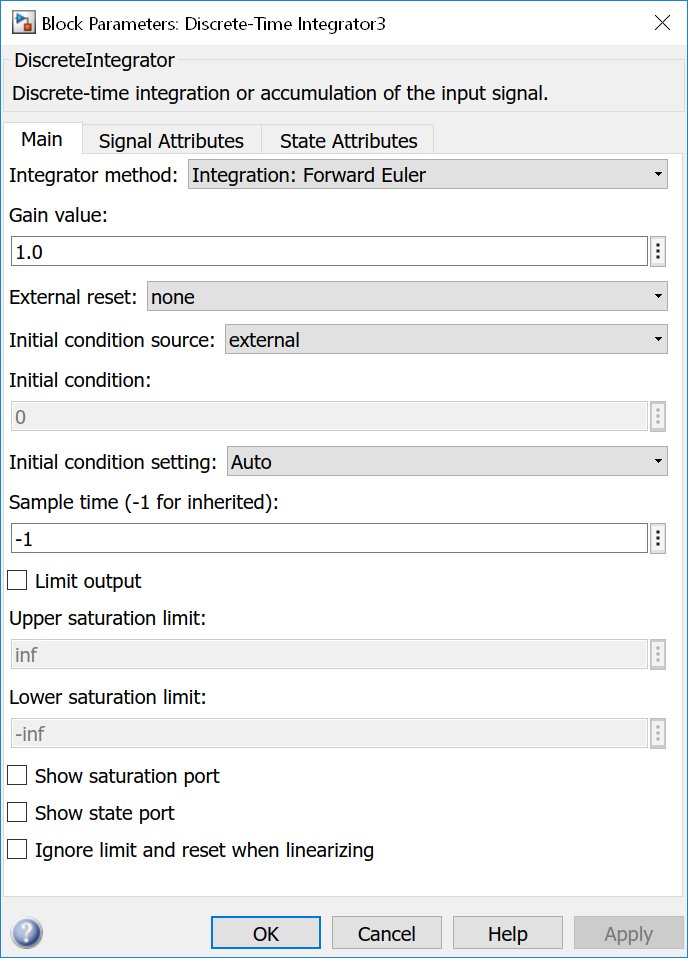
\includegraphics[width=0.7\textwidth]{figures/simulink_discrete_integrator.png}
		\caption{discrete time integrator settings}
		\label{fig:integrator}
\end{figure}	
\begin{figure}[H]
		\centering
		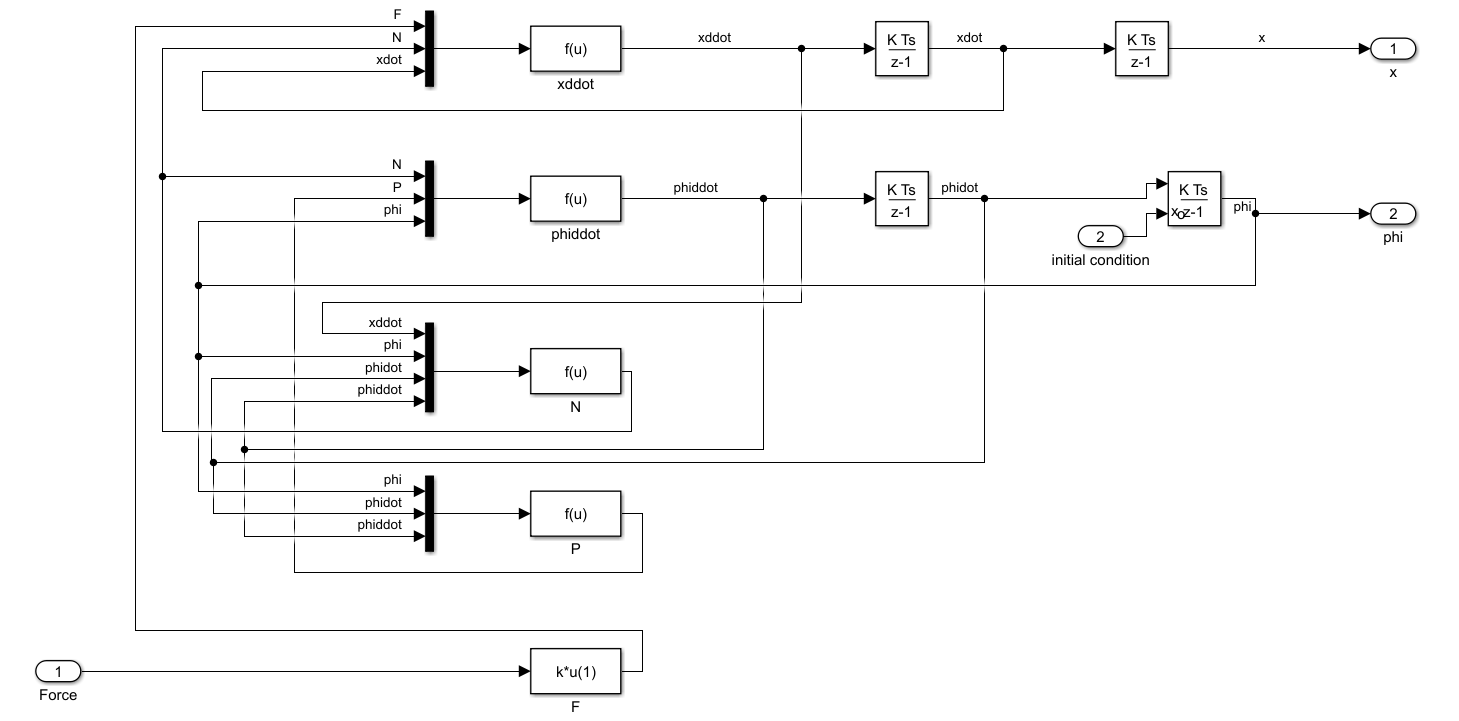
\includegraphics[width=0.7\textwidth]{figures/non_linear_discrete.png}
		\caption{Non linear discrete model in simulink}
		\label{fig:non_linear_continuous}
\end{figure}	

\subsection{Applying zero force to the system}
As a first test the model was tested with a constant of zero at its input. It would be expected to do nothing but stay upright since there are no external forces applied to the pendulum in the horizontal axis.	

\begin{figure}[H]
		\centering
		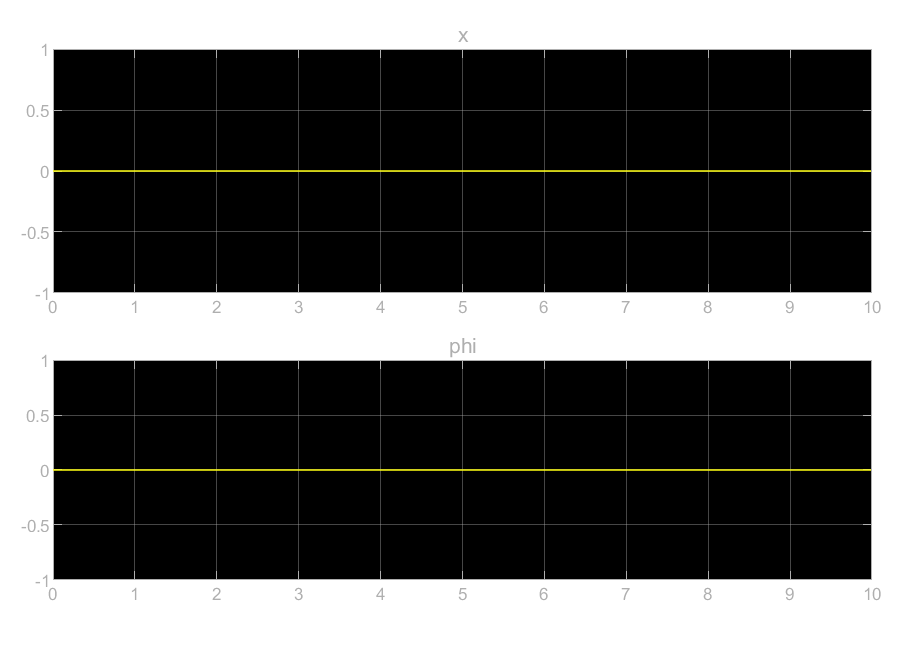
\includegraphics[width=0.7\textwidth]{figures/non_lin_disc_no_force.eps}
		\caption{Non linear discrete model simulation with zero force applied}
		\label{fig:non_linear_continuous}
\end{figure}
As a small test an initial step was applied to the system to see if it behaves correctly. The disturbance of the angle was accomplished by using the step function of simulink with an initial value of $10\cdot \frac{\pi}{180}$, which is 10° in radians.
As shown in Figure \ref{fig:sim_with_offset} the pendulum swings left and right and slowly loses height, so the model seems to be behaving correctly.
\begin{figure}[H]
		\centering
		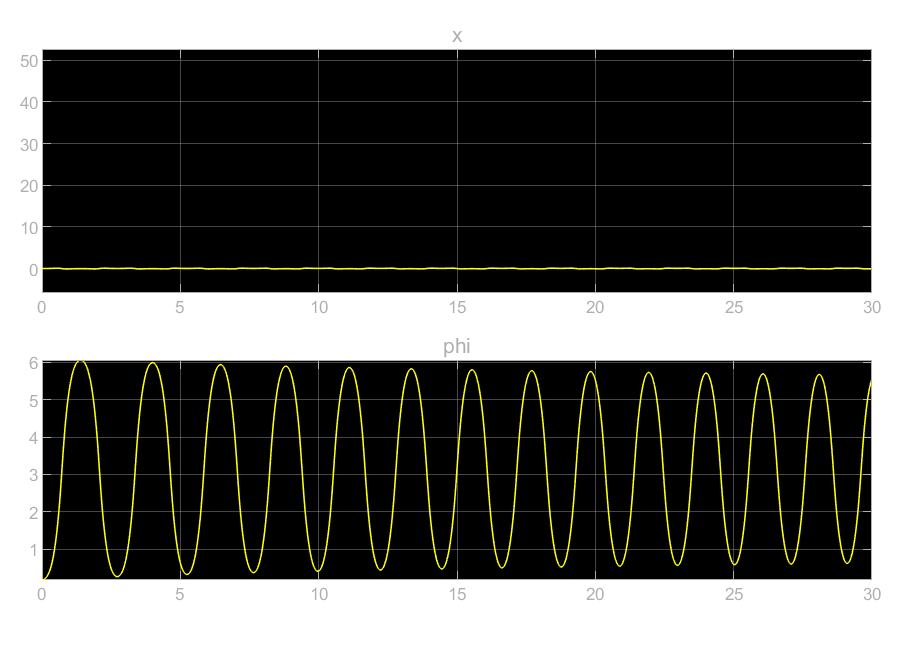
\includegraphics[width=0.7\textwidth]{figures/non_lin_disc_no_force_offset.eps}
		\caption{Non linear discrete model simulation with an offset step in the angle}
		\label{fig:sim_with_offset}
\end{figure}

\section{Linearization}
In order to further investigate the system for stability to make tuning the controller easier, it is mandatory to linearize the model. This is done by assuming that the slope of a sine wave is linear which of course is not the case but it is a valid approximation. The linearized equations are given by

	\begin{eqnarray}
		X\left(s\right)s^2=\frac{1}{M}\left(F\left(s\right)-mX\left(s\right)s^2+ml\Phi\left(s\right)s^2-bX\left(s\right)s\right)\\
		\Phi\left(s\right)s^2=\frac{1}{I}\ \left(mlX\left(s\right)s^2+mlg\Phi\left(s\right)-ml^2\Phi\left(s\right)s^2\right)
	\end{eqnarray}

From these equations the two transfer functions $G_1\left(s\right)=\frac{\Phi\left(s\right)}{F\left(s\right)}$ and $G_2\left(s\right)=\frac{X\left(s\right)}{F\left(s\right)}$ are to be found. This is simply a fact of rearranging the equations. \textbf{$G_1(s)$}
Solving equation 5 for $X(s)$:

\begin{eqnarray}
	X(s)\ s^2\ M=F(s)-mX(s)\ s^2+ml\Phi(s)\ s^2-bX(s)s \\
	X\left(s\right)s^2M=F\left(s\right)+ml\Phi\left(s\right)s^2+X\left(s\right)\left[-ms^2-bs\right] \\
	X\left(s\right)s^2M-X\left(s\right)\left[-ms^2-bs\right]=F\left(s\right)+ml\Phi\left(s\right)s^2 \\
	X\left(s\right)\left[s^2M+ms^2+bs\right]=F\left(s\right)+ml\Phi\left(s\right)s^2\\
	X\left(s\right)=\frac{F\left(s\right)+ml\Phi\left(s\right)s^2}{s^2M+ms^2+bs}
\end{eqnarray}

Inserting into equation 6 we get

\begin{eqnarray}
	\Phi\left(s\right)s^2=\frac{1}{I}\left[mls^2\cdot\frac{F\left(s\right)+ml\Phi\left(s\right)s^2}{s^2M+ms^2+bs}+mlg\Phi\left(s\right)-ml^2\Phi\left(s\right)s^2\right] \\
	\Phi\left(s\right)Is^2=mls^2\cdot\frac{F\left(s\right)+ml\Phi\left(s\right)s^2}{s^2M+ms^2+bs}+mlg\Phi\left(s\right)-ml^2\Phi\left(s\right)s^2 
	\\
	Is^2=mls^2\cdot\frac{\frac{F\left(s\right)}{\Phi\left(s\right)}+mls^2}{Ms^2+ms^2+bs}+mlg-ml^2s^2 \\
	Is^2=mls^2\cdot\frac{\frac{F\left(s\right)}{\Phi\left(s\right)}+mls^2}{Ms^2+ms^2+bs}+mlg-ml^2s^2 \\
	\frac{Is^2}{ml}=s^2\cdot\frac{\frac{F\left(s\right)}{\Phi\left(s\right)}+mls^2}{Ms^2+ms^2+bs}+g-ls^2 \\
	\frac{Is^2}{ml}=\frac{\frac{F\left(s\right)}{\Phi\left(s\right)}+mls^2}{M+m+\frac{b}{s}}+g-ls^2 \\
	\frac{F\left(s\right)}{\Phi\left(s\right)}=\left[\frac{I_s^2}{ml}-g+ls^2\right]\left[M+m+\frac{b}{s}\right]-mls^2 \\
	\frac{F\left(s\right)}{\Phi\left(s\right)}=\frac{MI}{ml}s^2+\frac{I}{l}s^2+\frac{Ib}{ml}s-gM-gm-\frac{gb}{s}+Mls^2+mls^2-mls^2 \\
	\frac{F\left(s\right)}{\Phi\left(s\right)}=s^2\left(\frac{MI}{ml}+\frac{I}{l}+Ml\right)+s\left(\frac{Ib}{ml}+lb\right)-gM-gm-\frac{gb}{s} \\
	\frac{\Phi\left(s\right)}{F\left(s\right)}=\frac{1}{s^2\left(\frac{MI}{ml}+\frac{I}{l}+Ml\right)+s\left(\frac{Ib}{ml}+lb\right)-gM-gm-\frac{gb}{s}} \\
	\frac{\Phi\left(s\right)}{F\left(s\right)}=\frac{s}{s^3\left(\frac{MI}{ml}+\frac{I}{l}+Ml\right)+s^2\left(\frac{Ib}{ml}+lb\right)+s(-gM-gm)-gb} 
	\\
	\frac{\Phi\left(s\right)}{F\left(s\right)}=\frac{s}{s^3\left(\frac{MI}{ml}+\frac{I}{l}+Ml\right)+s^2\left(\frac{Ib}{ml}+lb\right)+s\left(-gM-gm\right)-gb}
\end{eqnarray}


\textbf{$G_2(s)$}
Solving equation 6 for $\Phi(s)$:
\begin{eqnarray}
	\Phi\left(s\right)s^2=\frac{1}{I}\ \left(mlX\left(s\right)s^2+mlg\Phi\left(s\right)-ml^2\Phi\left(s\right)s^2\right)
	\\
	I\Phi\left(s\right)s^2=mlX\left(s\right)s^2+mlg\Phi\left(s\right)-ml^2\Phi\left(s\right)s^2
	\\
	\Phi\left(s\right)=\frac{mlX\left(s\right)s^2}{Is^2+ml^2s^2-mlg}
\end{eqnarray}

Inserting into the previously calculated transfer function:

\begin{eqnarray}
	\frac{\frac{mlX\left(s\right)s^2}{Is^2+ml^2s^2-mlg}}{F\left(s\right)}=\frac{s}{s^3\left(\frac{MI}{ml}+\frac{I}{l}+Ml\right)+s^2\left(\frac{Ib}{ml}+lb\right)+s(-gM-gm)-gb}
	\\
	\frac{X\left(s\right)}{F\left(s\right)}=\frac{Is^2+ml^2s^2-mlg}{mls^2}\cdot\frac{s}{s^3\left(\frac{MI}{ml}+\frac{I}{l}+Ml\right)+s^2\left(\frac{Ib}{ml}+lb\right)+s(-gM-gm)-gb}
	\\
	\frac{X\left(s\right)}{F\left(s\right)}=\frac{Is^2+ml^2s^2-mlg}{\ mls\cdot\left[s^3\left(\frac{MI}{ml}+\frac{I}{l}+Ml\right)+s^2\left(\frac{Ib}{ml}+lb\right)+s\left(-gM-gm\right)-gb\right]}
	\\
	\frac{X\left(s\right)}{F\left(s\right)}=\frac{s^2\left(I+ml^2\right)-mlg}{s^4\left(MI+Im+Mml^2\right)+s^3\left(Ib+m{bl}^2\right)+s^2\left(-gml\left[M+m\right]\right)-s\left(gbml\right)}
	\\
\end{eqnarray}

Our two transfer functions are therefore
\begin{eqnarray}
	G_1\left(s\right)=\frac{\Phi\left(s\right)}{F\left(s\right)}=\frac{s}{s^3\left(\frac{MI}{ml}+\frac{I}{l}+Ml\right)+s^2\left(\frac{Ib}{ml}+lb\right)+s(-gM-gm)-gb}
	\\
	G_2\left(s\right)=\frac{X\left(s\right)}{F\left(s\right)}=\frac{s^2\left(I+ml^2\right)-mlg}{s^4\left(MI+Im+Mml^2\right)+s^3\left(Ib+m{bl}^2\right)+s^2\left(-gml\left[M+m\right]\right)-s\left(gbml\right)}
\end{eqnarray}

To validate the calculations, the results were compared to the ones yielded in the online documentation\footnote{http://ctms.engin.umich.edu/CTMS/index.php?example=InvertedPendulum\&section=SystemModeling}.  The poles and zeros matched and therefore it can be assumed that the calculations are correct.

\section{Discretization linear model}

	\subsection{Forward Euler}
	
		\begin{eqnarray}
			z = e^{sT} \approx 1 + sT &\rightarrow& s \approx \frac{z - 1}{T}\\
			hallo &=& hallo
		\end{eqnarray}
	
	\subsection{Backward Euler}
		
		\begin{eqnarray}
			z = e^{sT} \approx \frac{1}{1 + sT} &\rightarrow& s \approx \frac{z - 1}{Tz}\\
			hallo &=& hallo
		\end{eqnarray}
	
	\subsection{Trapezoidal or Tustin}
	
		\begin{eqnarray}
			z = e^{sT} \approx \frac{1 + sT/2}{1 - sT/2} &\rightarrow& s \approx \frac{2\left( z - 1\right) }{T\left( z+1\right) }\\
			hallo &=& hallo
		\end{eqnarray}
		
	\subsection{Discretizing using Matlab}
	Matlab has a built in function $c2d()$ that can discretize a continuous time transfer function. It only requires the transfer function and the sample time as an input. We using 0.0001 seconds as the sampling time. The Matlab code is shown below:
\begin{lstlisting}
cart_n2 = (I+m*l^2)/q;
cart_n1 = 0;
cart_n0 = -g*m*l/q;
cart_d4 = 1;
cart_d3 = b*(I+m*l^2)/q;
cart_d2 = ((M + m)*m*g*l)/q;
cart_d1 = - b*m*g*l/q;
cart_d0 = 0;

pend_n1 = m*l/q;
pend_n0 = 0;
pend_d3 = 1;
pend_d2 = (b*(I + m*l^2))/q;
pend_d1 = -((M + m)*m*g*l)/q;
pend_d0 = -b*m*g*l/q;

P_cart = (cart_n2*s^2 + cart_n1*s + cart_n0)/(cart_d4*s^4 + cart_d3*s^3 + cart_d2*s^2 + cart_d1*s + cart_d0)
P_pend = (pend_n1*s + pend_n0)/(pend_d3*s^3 + pend_d2*s^2 + pend_d1*s + pend_d0)


%% discretizing the transfer functions
d_P_cart = c2d(P_cart, 0.0001)
d_P_pend = c2d(P_pend, 0.0001)

\end{lstlisting}

This script puts out the discrete transfer function
\begin{equation}
	\frac{2.273\cdot 10^{-8}z^2-1.377\cdot 10^{-13} z-2.273\cdot 10^{-8}}{z^3-3z^2+3z-1}
\end{equation}
\section{System analysis}
As a next step the transfer function of the systems shall be analysed using Matlab. This can be done using the command \textit{pzmap()}. 
\begin{lstlisting}
%Plotting poles and zeros 
figure
pzmap(P_cart, P_pend)
legend('cart','pendulum');

figure
pzmap(d_P_cart, d_P_pend)
legend('cart','pendulum');
\end{lstlisting}
This results in the following two figures.
\begin{figure}[H]
		\centering
		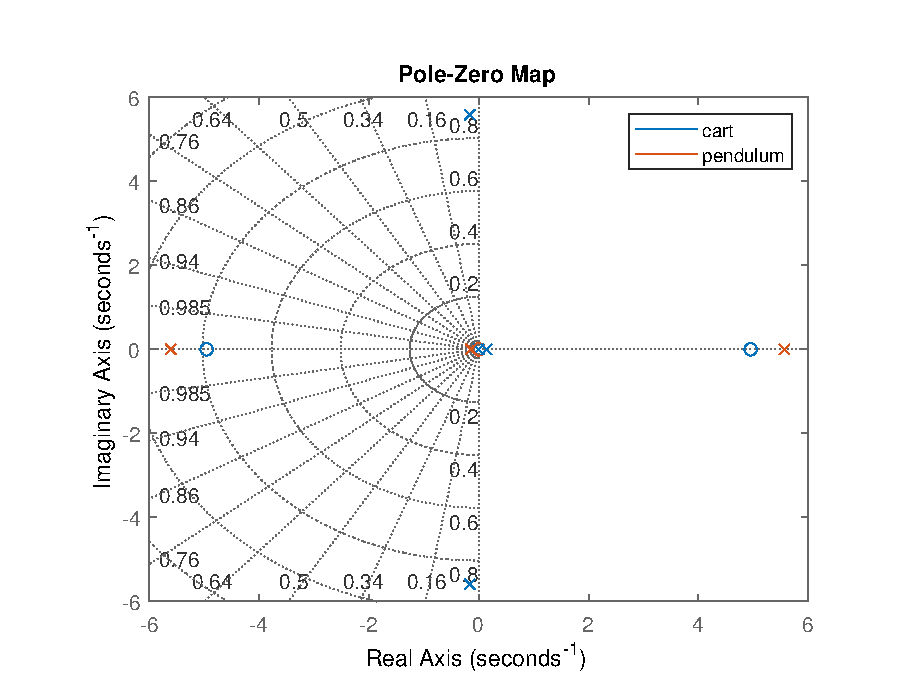
\includegraphics[width=0.7\textwidth]{figures/pzmap_cont.eps}
		\caption{pole and zero map of the continuous systems}
		\label{fig:pzmap_cont}
\end{figure}
\begin{figure}[H]
		\centering
		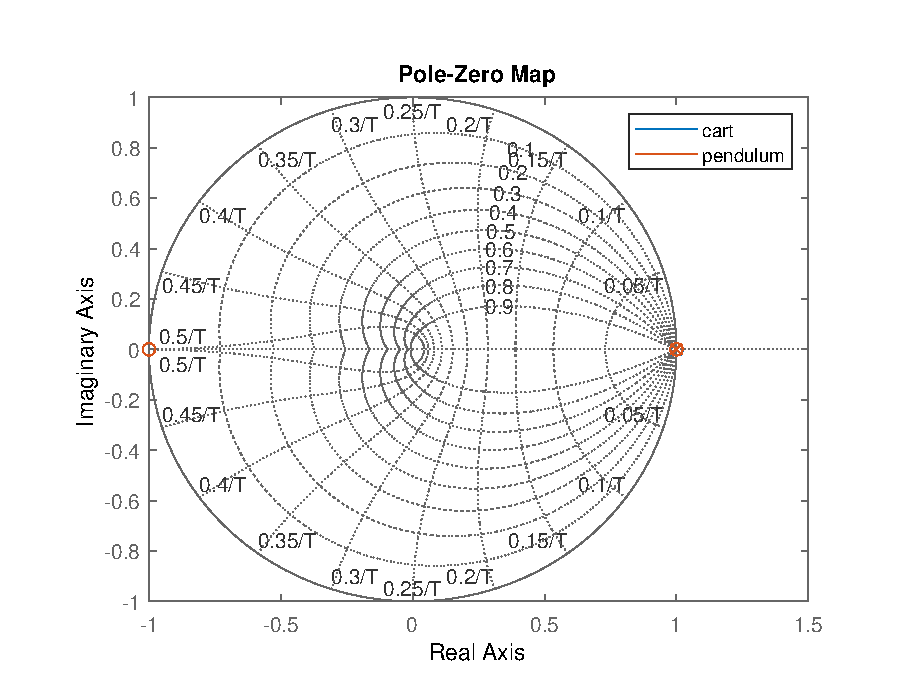
\includegraphics[width=0.7\textwidth]{figures/pzmap_disc.eps}
		\caption{pole and zero map of the discrete systems}
		\label{fig:pzmap_disc}
\end{figure}
As figure ~\ref{fig:pzmap_cont} and ~\ref{fig:pzmap_disc} show both the cart and the pendulum are unstable no matter if discretized or not. For the continuous system this can be detected because the poles do not all have a negative imaginary part. Looking at the discrete system at first glance it looks like all poles are within or at last at the unit circle. However after zooming in (see Figure ~\ref{fig:pzmap_disc_zoomed}) it appears that a pole is outside of the unit circle which results in an unstable system.
\begin{figure}[H]
		\centering
		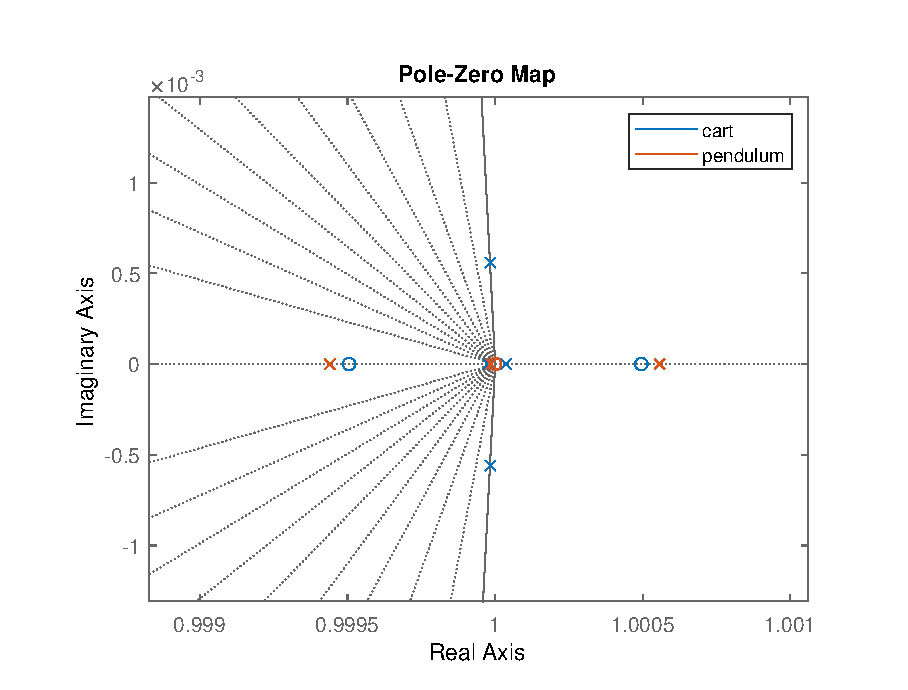
\includegraphics[width=0.7\textwidth]{figures/pzmap_disc_zoomed.eps}
		\caption{zoomed in pole and zero map of the discrete systems}
		\label{fig:pzmap_disc_zoomed}
\end{figure}
Next the both the discrete and the continuous model of the linearized model were implemented in simulink and tested next to each other. In order to get the denominator and the numerator of the transfer function for simulink, Matlabs \textit{tfdata} function was used.
\begin{figure}[H]
		\centering
		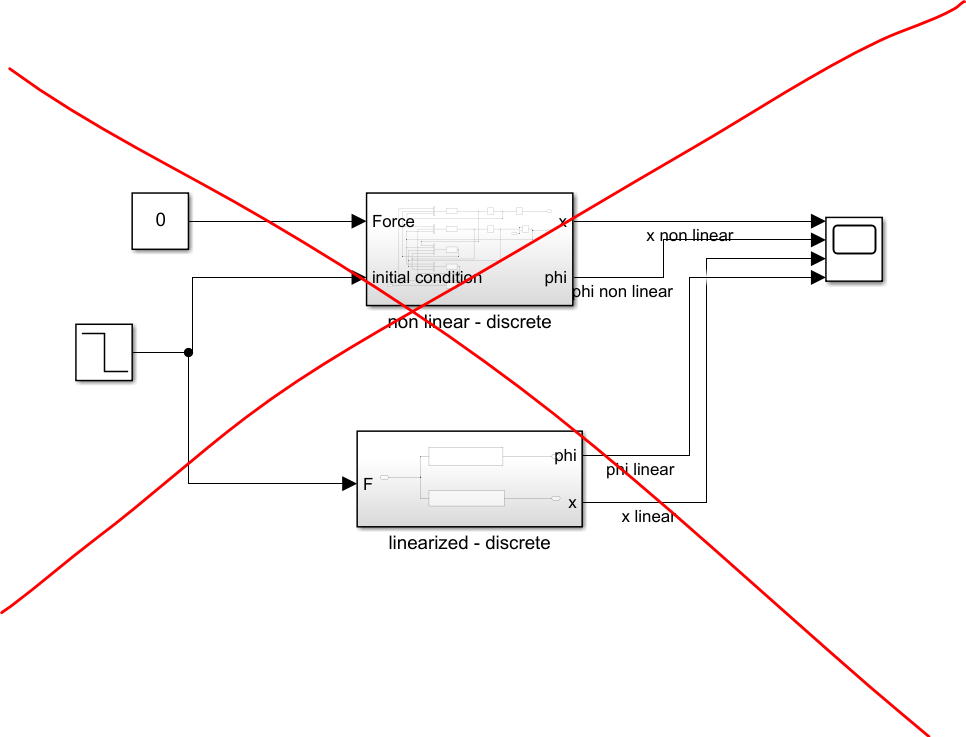
\includegraphics[width=0.7\textwidth]{figures/both_linearized_subsystems.png}
		\caption{discrete and continuous version of the linearized system}
		\label{fig:both_linearized_subsystems}
\end{figure}
\todo{Get right results}

\section{Control function}
Now that we have a working model of the pendulum we are going to have to control the cart in such a way, that it always keeps the pendulum upwards. For this purpose two models are going to be developed: one using the continuous plant and the other using the discrete one. The controller we'll be using is a simply PID controller that simulink offers. In addition a Kalman filter will be implemented in order to provide a more plausible vertical position coming form the plant.
Firstly, the provided Kalman filter was implemented using the Matlab function block and to test it the following model was built and simulated:
\begin{figure}[H]
		\centering
		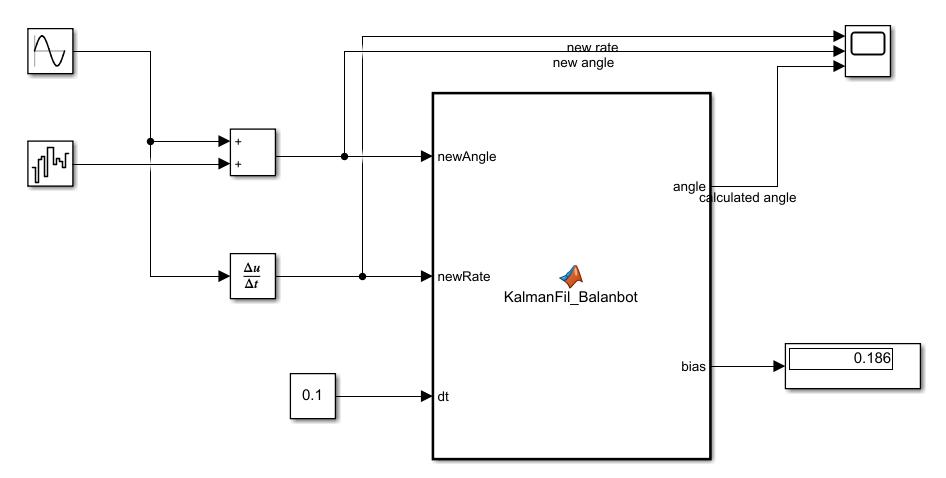
\includegraphics[width=0.7\textwidth]{figures/kalman_test.png}
		\caption{Kalman filter test model}
		\label{fig:kalman_test}
\end{figure}
\begin{figure}[H]
		\centering
		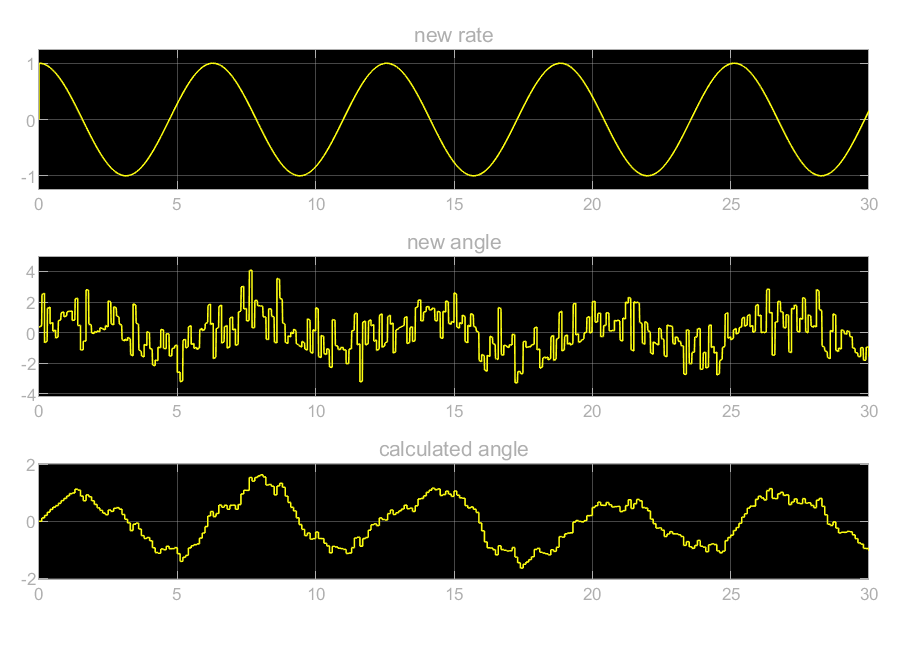
\includegraphics[width=0.7\textwidth]{figures/kalman_test_results.eps}
		\caption{Kalman filter test results}
		\label{fig:kalman_test_results}
\end{figure}
As Figure ~\ref{fig:kalman_test} shows, the filter works quite well, so we can move onto implementing the PID controllers. The complete simulink model with the controllers cna be seen in Figure ~\ref{fig:}


\part{Laboratory Session 07}


